\documentclass[a0,landscape]{a0poster}

\usepackage[margin=1cm]{geometry}
\usepackage{palatino, parskip, microtype, enumitem}
\usepackage{amsfonts, amsmath, amssymb, amsthm}
\usepackage[mathcal]{euscript}
\usepackage{xcolor, graphicx, tikz, qrcode, fontawesome5, stackengine}

% automatically creates a multicolumn layout
\usepackage{multicol}
\columnsep = .02\textwidth

\usepackage{ifdraft}

\title{Quasisymmetric harmonics of the exterior algebra}
\author{
  Nantel Bergeron, \thanks{\href{mailto:bergeron@yorku.ca}{bergeron@yorku.ca}}, 
  Kelvin Chan, \thanks{\href{mailto:ktychan@yorku.ca}{ktychan@yorku.ca}},
  Farhad Soltani, \thanks{\href{mailto:farhad.soltani91@gmail.com}{farhad.soltani91@gmail.com}}, \and
  Mike Zabrocki \thanks{\href{mailto:zabrocki@yorku.ca}{zabrocki@yorku.ca}}
}
\date{July 18, 2023}

% make editing easier
\usepackage{mdframed}
\newenvironment{postersection}[1][]
{% before 
  \begin{mdframed}[hidealllines=true]
    \IfNoValueTF{#1}{}{
      \begin{mdframed}[backgroundcolor=teal!0,hidealllines=true]
        \centering
        \large #1
      \end{mdframed}
    }
  }
  {% after
  \end{mdframed}
  \vspace{2em}
}

% shortcuts
% \newcommand{\qbinom}[2]{{\left[\begin{smallmatrix} {#1} \\ {#2} \end{smallmatrix} \right]}}
\newcommand{\qbinom}[2]{\genfrac{[}{]}{0pt}{}{#1}{#2}}
\newcommand{\email}[1]{\texttt{\footnotesize (#1)}}
\newcommand{\emoji}[1]{\faIcon{#1}}
\newcommand{\exampleone}{
  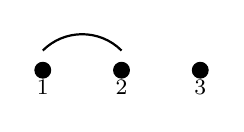
\begin{tikzpicture}
    \filldraw (1,0) circle (0.1) node[below] {\footnotesize $1$};
    \filldraw (2,0) circle (0.1) node[below] {\footnotesize $2$};
    \filldraw (3,0) circle (0.1) node[below] {\footnotesize $3$};
    \begin{scope}[shift={(1,0.25)}]
      \draw[thick] (0, 0) arc (135:45:{sqrt(2)/2});
    \end{scope}
  \end{tikzpicture}
}
\newcommand{\exampletwo}{
  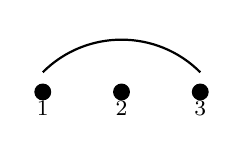
\begin{tikzpicture}
    \filldraw (1,0) circle (0.1) node[below] {\footnotesize $1$};
    \filldraw (2,0) circle (0.1) node[below] {\footnotesize $2$};
    \filldraw (3,0) circle (0.1) node[below] {\footnotesize $3$};
    \begin{scope}[shift={(1,0.25)}]
      \draw[thick] (0, 0) arc (135:45:{sqrt(8)/2});
    \end{scope}
  \end{tikzpicture}
}
\newcommand{\examplethree}{
  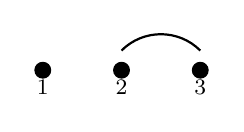
\begin{tikzpicture}
    \filldraw (1,0) circle (0.1) node[below] {\footnotesize $1$};
    \filldraw (2,0) circle (0.1) node[below] {\footnotesize $2$};
    \filldraw (3,0) circle (0.1) node[below] {\footnotesize $3$};
    \begin{scope}[shift={(2,0.25)}]
      \draw[thick] (0, 0) arc (135:45:{sqrt(2)/2});
    \end{scope}
  \end{tikzpicture}
}

\begin{document}

%--------------------------------------------------
%
% title block
%
%--------------------------------------------------
% takes up the entire top of the page
\begin{mdframed}[backgroundcolor=teal!5, hidealllines=true]
  % \centering
  % \raggedright
  % \hfill{}
  \hspace{.1\textwidth}
  \begin{minipage}{.7\textwidth}
    {\veryHuge \textcolor{black}{Quaisymmetric harmonics of the exterior algebra} \quad
    \qrcode[height=1in]{https://www.mat.univie.ac.at/~slc/wpapers/FPSAC2023/32.pdf} }
    \medskip

    {Nantel Bergeron \email{bergeron@yorku.ca}, Kelvin Chan \email{\footnotesize ktychan@yorku.ca}, Farhad Soltani \email{farhad.soltani91@gmail.com}, Mike Zabrocki \email{zabrocki@yorku.ca}} 

    {York University, Toronto, Canada} 
  \end{minipage}
  \quad
  % \begin{minipage}{.1\textwidth}
  %   Nantel Bergeron
  %
  %   Kelvin Chan
  %
  %   Farhad Soltani
  %
  %   Mike Zabrocki
  %
  %   {York University, Toronto, Canada} 
  % \end{minipage}
  \quad
  \begin{minipage}{.2\textwidth}
    % Fields https://www.fields.utoronto.ca/generalinfo/Acknowledging-Fields-Institute-Funding
    % YORK  https://www.yorku.ca/brand/py_community_area/brand-building-blocks/logos/    
    
\includegraphics[height=1in]{logo_york.eps} \hspace{2em}
    % \includegraphics[height=1in]{logo_fields.eps}\hspace{2em}
    % NSERC https://www.nserc-crsng.gc.ca/NSERC-CRSNG/acknowledgement_and_logos-mention_et_logos/index_eng.asp
    
\includegraphics[height=1in]{logo_nserc.eps}\hspace{2em}
  \end{minipage}
\end{mdframed}

\medskip
\hrulefill{}

%--------------------------------------------------
%
% content
%
%--------------------------------------------------
\begin{multicols}{3}
  \begin{postersection}[Overview \emoji{shipping-fast}]
      \begin{center}
        
\begin{tikzpicture}[scale=2]
          \foreach \x in {0,...,9} {
            \filldraw (\x,0) circle (0.1);
          }

          % small arcs
          \foreach \x in {1,5,8} {
            \begin{scope}[shift={(\x,0.25)}]
              \draw[thick] (0, 0) arc (135:45:{sqrt(2)/2});
            \end{scope}
          }

          % larger arcs
          \foreach \x in {4} {
            \begin{scope}[shift={(\x,0.25)}]
              \draw[thick] (0, 0) arc (135:45:{3*sqrt(2)/2});
            \end{scope}
          }
        \end{tikzpicture}
      \end{center}
      \bigskip

      What do the \emph{coinvariants} look like in the setting of the exterior algebra with a \emph{quasisymmetric} action of $\mathcal{S}_{n}$? The short answer: $\{0,1\}$-Ballot sequences and more! 
      \[
        \mathrm{Hilb}_{R_{n}/I_{n}}(q) = \sum_{k = 0}^{\lfloor n/2 \rfloor} f^{(n-k,k)} q^{k}.
      \]
    \end{postersection}
    
    \begin{postersection}[The History \emoji{history}]
      % Many coinvariant quotients feature rich combinatorial connections.  One well-known example is the coinvariant ring of the symmetric group
      % \[ \mathbb{Q}[x_{1},\dots,x_{n}] / \langle Sym_{n}^{+} \rangle \]
      % whose dimension is $n!$.  It is the quotient of the polynomial ring $\mathbb{Q}[x_{1},\dots,x_{n}]$ in commuting variables by the ideal generated by the symmetric polynomials with no constant term.  As a symmetric group $\mathcal{S}_{n}$ representation, this quotient is naturally graded and is well-known to be isomorphic to the regular representation.  Its graded Hilbert series is the $q$-factorial.  Many useful bases of this space have been found by studying combinatorics related to permutations.  This line of inquiry has been generalized to reveal many interesting combinatorics, including the famous $q,t$-Catalan numbers and the now Shuffle Theorem.

      The ring of quasisymmetric function $QSym_{n}$ includes the ring of symmetric function. Many combinatorial structures of $QSym_{n}$ parallel that of $Sym_{n}$. Hivert described an action of the Temperley-Lieb algebra $TL_{n}$, thought of as a quotient of the symmetric group algebra, on $\mathbb{Q}[x_{1},\dots,x_{n}]$ making $QSym_{n}$ an isotypic trivial representation of $TL_{n}$. In 2003, Avel, F. Bergeron, and the first author studied $QSym$ coinvariant spaces 
      \[ \mathbb{Q}[x_{1},\dots,x_{n}] / \langle QSym_{n}^{+} \rangle \]
      obtained by replacing the ideal of symmetric functions with no constant terms with the ideal of quasisymmetric functions with no constant terms. They developed a basis $\{ G_{\pi} \}$ of the polynomial ring indexed by lattice paths and gave a criterion for monomial membership of $\langle QSym_{n}^{+} \rangle$ by whether the indexing path crosses the diagonal.
      \begin{center}
        \medskip
        \begin{tikzpicture}
          \begin{scope}[shift={(-5,0)}]
          
          \draw[dotted] (0,0) -- (8,8);
          \foreach \x in {0,...,8} {
            \foreach \y in {\x,...,8} {
              \filldraw[gray!50] (\x,\y) circle (0.05);
            }
          }

          \draw[thick] (0,0) --++(0,2) --++(2,0) --++(0,3) --++(2,0) --++(0,1) --++(1,0);

          \node[above right] at (2,0) {\footnotesize $x_{3}^{2} x_{6}^{2} x_{7} \notin \langle QSym_{n}^{+} \rangle$.};
          \end{scope}

          \begin{scope}[shift={(5,0)}]
            \foreach \x in {0,...,8} {
              \foreach \y in {\x,...,8} {
                \filldraw[gray!50] (\x,\y) circle (0.05);
              }
            }
            \draw[dotted] (0,0) -- (8,8);

            \draw[thick] (0,0) --++(0,3) --++(1,0) --++(0,1) --++(3,0);
            \draw[red, thick] (4,4) -- (6,4) --++(0,2);
            \draw[thick] (6,6) --++(0,2) --++(1,0);

            \node[above right] at (2,0) {\footnotesize $x_{4} x_{5}^{5} x_{9} \in \langle QSym_{n}^{+} \rangle$.};
          \end{scope}
          
        \end{tikzpicture}
        \medskip
      \end{center}
      Surprisingly, the dimensions of the $QSym$ coinvariants are equal to the Catalan numbers!

    \end{postersection}

    \begin{postersection}[The Setup]
      Motivated by recent development in coinvariant theory involving Fermionic (anticommuting) variables, we study the $QSym$ coinvariant spaces of the exterior algebra
      \[
        EQC_{n} = R_{n} / I_{n}.
      \]

      \begin{itemize}
        \item The exterior algebra is $R_{n} = \mathbb{Q}[\theta_{1}, \dots, \theta_{n}]$ with $\theta_{i} \theta_{j} = - \theta_{j} \theta_{i}$.
        \item Index monomials by sets $\theta_{\{1,3,5\}} = \theta_{1} \theta_{3} \theta_{5}$.
        \item Extend Hivert's $\mathcal{S}_{n}$-action: Act by permutation but ignore signs
          \[
            (2,5) \cdot \theta_{\{1,3,5\}} = \theta_{(2,5) \{1,3,5\}} = \theta_{\{1,2,3\}} = \theta_{1} \theta_{2} \theta_{3}.
          \]
        \item Invariant polynomials are called \emph{quasisymmetric}. A basis consists of
          \begin{align*}
            F_{1^{k}} 
            &=\sum_{\substack{A \subseteq [n]\\|A|=k}} \theta_{A}, \quad k = 1,\dots,n \\
            \intertext{In $\mathbb{Q}[\theta_{1}, \theta_{2}, \theta_{3}]$,}
            F_{1} 
            &= \theta_{1} + \theta_{2} + \theta_{3},\\
            F_{11} 
            &= \theta_{1}\theta_{2} + \theta_{1}\theta_{3} + \theta_{2}\theta_{3},\\
            F_{111} 
            &= \theta_{1}\theta_{2}\theta_{3}
          \end{align*}
        \item The quasisymmetric invariant ideal is $I_{n} = \langle F_{1}, \dots, F_{n} \rangle$. 
      \end{itemize}
    \end{postersection}

    \begin{postersection}[Detour to symmetric invariants]
      Act by permutations but with signs.
      \[
        (2,5) \theta_{\{1,3,5\}} = (2,5) \theta_{1} \theta_{3} \theta_{5} = \theta_{1} \theta_{3} \theta_{2} = - \theta_{1} \theta_{2} \theta_{3} = - \theta_{\{1,2,4\}}.
      \]

      The symmetric invariants $\mathbb{Q}\{ \theta_{1} + \cdots + \theta_{n} \}$ form a $1$-dimensional subspace.
      \[ (1 + (1,2)) \cdot \theta_{1} \theta_{2} = \theta_{1} \theta_{2} - \theta_{1} \theta_{2} = 0. \]
      % The symmetric invariants $\mathbb{Q}\{ \theta_{1} + \cdots + \theta_{n} \}$ form a $1$-dimensional subspace  because $e_{k}(\theta_{1}, \dots, \theta_{n}) = 0$ if $k \ge 2$. \[ (1 + (1,2)) \cdot \theta_{1} \theta_{2} = \theta_{1} \theta_{2} - \theta_{1} \theta_{2} = 0. \]
      
      
      A parallel to the classic coinvariant story: 
      %We have a parallel statement to that of the classic coinvariant theory that $\mathbb{Q}[x_{1},\dots,x_{n}]$ is free over $Sym_{n}$. 

      \textbf{Theorem}. The exterior algebra $R_{n}$ is free over its \emph{symmetric} polynomials. 
    \end{postersection}
    
    \begin{postersection}[The structure of $I_{n}$]
      We extend a result of Fishel, Lapointe and Pinto by determining the structural coefficients of $\mathrm{QSym}_{n}$. 

      \textbf{Theorem}. The algebra $\mathrm{QSym}_{n} = \mathbb{Q}[F_{1}, \dots, F_{1^{n}}]$ is commutative and
      \[
        F_{1^{r}}F_{1^{s}} = 
        \begin{cases}
          \displaystyle
          \binom{\lfloor\frac{r+s}{2}\rfloor}{\lfloor\frac{r}{2}\rfloor} F_{1^{r+s}} & \text{if } rs \equiv 0 \pmod{2} \\
          0 & \text{otherwise}
        \end{cases}.
      \]

      That means the ideal $I_{n}$ is very simple! 
      \begin{equation} \label{eq:In-generators}
        I_{n} = \langle F_{1}, F_{11} \rangle.
      \end{equation}
    \end{postersection}

    \begin{postersection}[Harmonics]
      Let $R_{n}$ act on itself by partial differentiation. Differential operators $\partial_{\theta_{k}}$ also anticommute. 
      \[
        \partial_{\theta_{1}} \theta_{1}\theta_{2} = \theta_{2} \quad\text{and}\quad \partial_{\theta_{2}} \theta_{1} \theta_{2} = \theta_{1} ( - \partial_{\theta_{2}} ) \theta_{2} = \theta_{1}.
      \]

      The harmonics are
      \[
        EQH_{n} =  \Big\{ q \in R_n :  \quad\sum_{1\le i\le n} \partial_{\theta_i}q= 0 \quad\hbox{ and  }\quad \sum_{1\le i<j\le n} \partial_{\theta_j}\partial_{\theta_i}q= 0 \Big\}~.
      \]
      And $EQC_{n} \cong EQH_{n}$.

      Non-crossing pairings build harmonic polynomials.
      \begin{center}
        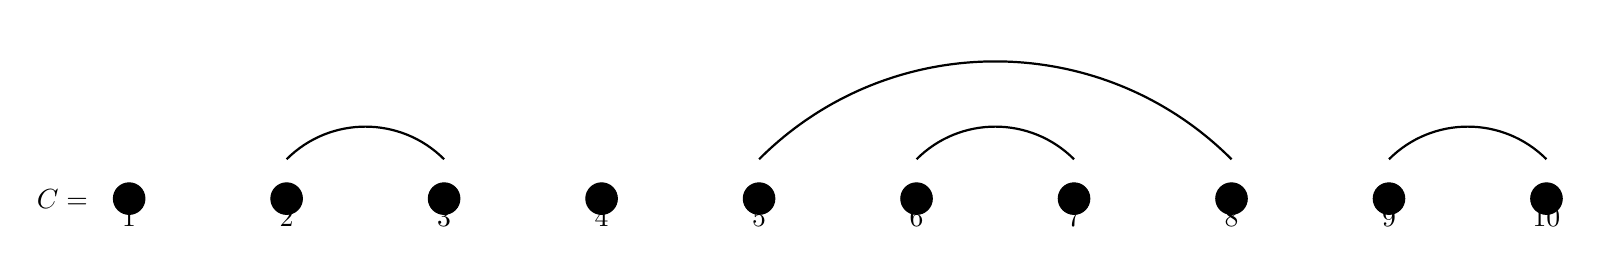
\begin{tikzpicture}[scale=2]
          \foreach \x in {1,...,10} {
            \filldraw (\x,0) circle (0.1);
            \node[below] at ({\x},0) {$\x$};
          }

          % small arcs
          \foreach \x in {2,6,9} {
            \begin{scope}[shift={(\x,0.25)}]
              \draw[thick] (0, 0) arc (135:45:{sqrt(2)/2});
            \end{scope}
          }

          % larger arcs
          \foreach \x in {5} {
            \begin{scope}[shift={(\x,0.25)}]
              \draw[thick] (0, 0) arc (135:45:{3*sqrt(2)/2});
            \end{scope}
          }

          \node[left] at (0.8,0) {$C = $};
        \end{tikzpicture}
      \end{center}
      \[
        \Delta_{C} = (\theta_{3} - \theta_{2}) (\theta_{7}  - \theta_{6}) (\theta_{8} - \theta_{5}) ( \theta_{10} - \theta_{9} ).
      \]

      However, they are not linearly independent:
      \[
        \Delta_{\exampleone} - \Delta_{\exampletwo} + \Delta_{\examplethree} = 0.
      \]
    \end{postersection}

    \begin{postersection}[Ballot sequences and non-crossing pairing]
      A $\{0,1\}$-sequence is ballot (aka Yamanouchi) if every prefix has at least as many $0$'s as $1$'s.

      \begin{center}
      \textcolor{teal}{\faIcon[regular]{thumbs-up}} Yes ballot: $0010001101$. 
      \hspace{2em}
      \textcolor{magenta}{\faIcon[regular]{thumbs-down}} Not ballot: ${\color{magenta}011}0001101$.
      \end{center}

      From ballot sequence to non-crossing pairings.
      \begin{center}
        \begin{tikzpicture}[scale=2]
          \begin{scope}
            \node at (1,0) {$0$};
            \node at (2,0) {$0$};
            \node at (3,0) {$1$};
            \node at (4,0) {$0$};
            \node at (5,0) {$0$};
            \node at (6,0) {$0$};
            \node at (7,0) {$1$};
            \node at (8,0) {$1$};
            \node at (9,0) {$0$};
            \node at (10,0) {$1$};

            \node[left] at (0,0) {$\alpha=$};
          \end{scope}
          \begin{scope}[shift={(0,-1)}]
            \node at (1,0) {$($};
            \node at (2,0) {$($};
            \node at (3,0) {$)$};
            \node at (4,0) {$($};
            \node at (5,0) {$($};
            \node at (6,0) {$($};
            \node at (7,0) {$)$};
            \node at (8,0) {$)$};
            \node at (9,0) {$($};
            \node at (10,0) {$)$};
          \end{scope}
          \begin{scope}[shift={(0,-3)}]
          \foreach \x in {1,...,10} {
            \filldraw (\x,0) circle (0.1);
            \node[below] at ({\x},0) {$\x$};
          }
          % small arcs
          \foreach \x in {2,6,9} {
            \begin{scope}[shift={(\x,0.25)}]
              \draw[thick] (0, 0) arc (135:45:{sqrt(2)/2});
            \end{scope}
          }

          % larger arcs
          \foreach \x in {5} {
            \begin{scope}[shift={(\x,0.25)}]
              \draw[thick] (0, 0) arc (135:45:{3*sqrt(2)/2});
            \end{scope}
          }
          \node[left] at (0,0) {$C(\alpha)=$};
          \end{scope}
        \end{tikzpicture}
        
      \end{center}
      
      Interpret a $0$ as a North step and a $1$ as an East step:
      \begin{center}
        \begin{tikzpicture}
          \begin{scope}[shift={(-5,0)}]
            \draw[dotted] (0,0) -- (8,8);
            \foreach \x in {0,...,8} {
              \foreach \y in {\x,...,8} {
                \filldraw[gray!50] (\x,\y) circle (0.05);
              }
            }

            \draw[thick] (0,0) -- ++(0,2) -- ++(1,0) -- ++(0,3) -- ++(2,0) -- ++(0,1) -- ++(1,0);
            \node[above right] at (2,0) {$0010001101$};
          \end{scope}
        \end{tikzpicture}
      \end{center}
      
      \textbf{Theorem}. $\{ \Delta_{C(\alpha)} : \alpha \text{ is a ballot sequence } \}$ is linearly independent in $QHC_{n}$.
    \end{postersection}
    
    \begin{postersection}[A linear basis of $R_{n}$]
      Recursively define a family of polynomials analogous to that of Avel-Bergeron-Bergeron.
      \begin{align*}
        G_{1^{s}0^{n-s}} &= F_{1^{s}} \\
        G_{u \mathbf{\color{teal}0} 1^{s} 0^{n-k-s}} &= G_{u 1^{s} 0^{n-k-s}\mathbf{\color{teal}0}} - (-1)^{\text{\# of $1$'s in $u$}} \theta_{k} G_{u 1^{s-1} 0^{n-k-s+1}\mathbf{\color{teal}0}},
      \end{align*}
      where $k = \ell(u)+1$ is the position of the right-most non-trailing $0$.

      The idea is to recursively get ``closer'' to $F_{1^{k}}$. Examples:
      \begin{itemize}
        \item Indexed by a non-ballot sequence:
          \begin{align*} 
            G_{01\mathbf{\color{teal}0}110} 
          & = G_{01110\mathbf{\color{teal}0}} - (-1)^{1} \theta_{3} G_{01100\mathbf{\color{teal}0}} \\
          &= (G_{111000} - \theta_{1} G_{110000}) + \theta_{3}(G_{110000} - \theta_{1}G_{100000})
          \end{align*}
        \item Indexed by a ballot sequence:
          \begin{align*}
            G_{00110\mathbf{\color{teal}0}} 
            &= G_{01100\mathbf{\color{teal}0}} - \theta_{2} G_{01000\mathbf{\color{teal}0}} \\
            &= (G_{110000} - \theta_{1} G_{100000}) - \theta_{2}(G_{100000} - \theta_{1}G_{000000}) \\
            &= \theta_3 \theta_4 + \theta_3 \theta_5 + \theta_3 \theta_6 + \theta_4 \theta_5 + \theta_4 \theta_6 + \theta_5 \theta_6.
          \end{align*}
      \end{itemize}
      
      \textbf{Theorem}. 
      \begin{enumerate}
       \item The lexicographical leading term of $G_{\alpha}$ is $\theta^{\alpha}$.
       \item The set $\{ G_{\alpha} : \alpha \text{ is a ballot sequence }\}$ is a basis for $EQC_{n}$.
      \end{enumerate}
      
    \end{postersection}
    

    \begin{postersection}[Acknowledgement]
      We acknowledge the support of the Natural Sciences and Engineering Research Council of Canada (NSERC), the Fields Institute, and York University, Canada.
    \end{postersection}
    
  \end{multicols}
\end{document}

